% the following line is added to eliminate warnings about fonts on Mac
\PassOptionsToPackage{quiet}{fontspec} 

% use ctexarticle and include own package hw-cn.sty
\documentclass[]{ctexart}
\usepackage{hw-cn}

\usepackage{inputenc}
\usepackage{amsfonts,amsmath,amscd,amssymb,amsthm}
\usepackage{latexsym,bm}
\usepackage{cite}
\usepackage{mathtools,mathdots,graphicx,array}
\usepackage{fancyhdr}
\usepackage{lastpage}
\usepackage{color}
\usepackage{enumitem}
\usepackage{diagbox}
\usepackage{xcolor,tcolorbox,tikz,tkz-tab,mdframed,tikz-cd}
\usepackage{framed}
\usepackage{verbatim}
\usepackage{extarrows}
\usepackage{fontspec}
\usepackage{subfigure}
\usepackage{float}
\usepackage{graphicx}
\usepackage{listings}
\usepackage{hyperref}
\usepackage{makecell}
\usepackage{bbding}


\newcommand\course{智能感知认知实践}
\newcommand\labnumber{任务}
\newcommand\name{孙一林}
\newcommand\stuID{520030910361}

\pagestyle{fancyplain}
\headheight 25pt
\lhead{\name \\ \stuID}
\chead{\textbf{\Large 语言模型\labnumber}}
\rhead{\course \\ \today}



\begin{document}

\section{提交文件简要说明}
本次实验代码在超算中提供的代码框架基础上进行了更改。提交文件夹中,\texttt{checkpoint}目录下是实验运行结果,
包括各种模型在不同超参数下的实验日志,不同模型以不同的文件夹区分,而模型超参数则保存在\texttt{.txt}文件名中。
\texttt{tensorboard}文件夹下则保存了不同模型、参数下\texttt{SummaryWriter}的运行日志,即\texttt{events.out.tfevents.}前缀文件。
\section{各语言模型结构的理解}

\subsection{RNN}
在时间序列数据中,当前的观察依赖于之前的观察,因此观察之间不是相互独立的。
然而,传统的神经网络将每个观察视为独立的,这就导致了循环神经网络(RNN)的兴起,
它通过包含数据点之间的依赖关系将记忆的概念引入神经网络。

通过反馈回路,一个RNN单元的输出也被同一单元用作输入。因此,每个RNN都有两个输入:过去和现在。使用过去的信息会产生短期记忆。
在每个单元格中,当前时间步的输入、前一时间步的隐藏状态和偏置组合,然后通过激活函数限制以确定当前时间的隐藏状态步。
由于其短期记忆,RNN可以处理顺序数据并识别历史数据中的模式。此外,RNN能够处理不同长度的输入。

RNN存在梯度下降消失的问题。在这种情况下,用于在反向传播期间更新权重的梯度变得非常小。将权重与接近于零的梯度相乘会阻止网络学习新的权重。停止学习会导致RNN忘记在较长序列中看到的内容。梯度下降消失的问题随着网络层数的增加而增加。

由于RNN仅保留最近的信息,所以该模型在考虑过去的观察时会出现问题。因此,RNN只有短期记忆而没有长期记忆。

此外,由于RNN使用反向传播及时更新权重,网络也会遭受梯度爆炸的影响,如果使用ReLu激活函数,则会受到死亡ReLu单元的影响。
前者可能会导致收敛问题,而后者会导致停止学习。

\subsection{LSTM}
LSTM是一种特殊类型的RNN,它解决了RNN会梯度消失的问题。
LSTM的关键是单元状态,它从单元的输入传递到输出。单元状态允许信息沿着整个链流动,仅通过三个门进行较小的线性动作。因此,单元状态代表LSTM的长期记忆。这三个门分别称为遗忘门、输入门和输出门。这些门用作过滤器并控制信息流并确定保留或忽略哪些信息。
遗忘门决定了应该保留多少长期记忆。为此,使用了一个sigmoid函数来说明单元状态的重要性。输出在0和1之间变化,0即不保留任何信息;1则保留单元状态的所有信息。
输入门决定将哪些信息添加到单元状态,从而添加到长期记忆中。
输出门决定单元状态的哪些部分构建输出。因此,输出门负责短期记忆。
总的来说,状态通过遗忘门和输入门更新。
LSTM的主要优点是它可以捕获序列的长期和短期模式,但由于结构更复杂,LSTM的计算成本更高,从而导致训练时间更长。

\subsection{GRU}
与LSTM类似,GRU解决了简单RNN的梯度消失问题。然而,与LSTM的不同之处在于GRU使用较少的门并且没有单独的内部存储器,即单元状态。因此,GRU完全依赖隐藏状态作为记忆,从而导致更简单的架构。
重置门负责短期记忆,因为它决定保留和忽略多少过去的信息。
更新门负责长期记忆,可与LSTM的遗忘门相媲美。
当前时间步的隐藏状态是基于两个步骤确定的:
首先,确定候选隐藏状态。候选状态是当前输入和前一时间步的隐藏状态以及激活函数的组合。前一个隐藏状态对候选隐藏状态的影响由重置门控制。
第二步,将候选隐藏状态与上一时间步的隐藏状态相结合,生成当前隐藏状态。先前的隐藏状态和候选隐藏状态如何组合由更新门决定。
如果更新门给出的值为0,则完全忽略先前的隐藏状态,当前隐藏状态等于候选隐藏状态。如果更新门给出的值为1,则相反。
由于与LSTM相比有着更简单的架构,GRU的计算效率更高,训练速度更快,只需要更少的内存。
此外,GRU已被证明对于较小的序列更有效。
由于GRU没有单独的隐藏状态和细胞状态,因此它们可能无法像LSTM那样考虑过去的观察结果。

\subsection{Transformer}
Transformer是一种基于注意力机制的序列到序列模型,它在2017年由Vaswani等人提出。Transformer的主要优点是它能够并行处理输入序列,而不是像RNN那样顺序处理。这使得Transformer比RNN更快,更容易训练。此外,Transformer还能够捕获长期依赖性,而无需使用RNN或CNN。
Transformer没有了序列,将输入的语句当作一个整体,输入到embedding层中,因此有了并行计算的能力,
不再强调输入序列次序。因此,也就没有长依赖的问题。
位置编码是一种向输入嵌入中添加位置信息的技术,它使模型能够理解输入中某些部分在整个输入中的位置。
需要注意的是,transformer中不再使用循环结构,因此必须以不同的方式添加位置信息,而这正是通过位置编码来实现的。
这种方式的优点也是解决了序列顺序依赖的同时,也能将位置信息考虑在模型中。
自注意力机制是transformer中最常见的结构。自注意力机制是Transformer的一个核心组件。
与之前的注意力机制不同的是,可以将序列中不同位置之间的依赖关系进行建模,不需要依赖于时间的顺序,因此可以更好地处理长序列。

\newpage
\section{实验和超参数分析}
\subsection{同一参数下模型性能对比}
由于本实验中我们研究了大量的不同语言模型,为了能够对比其性能的差异,
应保持参数的一致性。这里列举了两种不同参数配置下的实验结果。
\begin{table}[H]
  \centering
  \begin{tabular}{|c|c|c|c|c|c|c|c|c|c|c|c|c|}
    \hline
      \diagbox{评估指标}{模型选取}
      &RNN(Relu)&RNN(Tanh)&LSTM&GRU&Transformer\\
      \hline
      Test Loss&NA&5.26&4.95&5.26&6.55\\
      \hline
      Perplexity&NA&192.27&141.38&192.27&700.61\\
      \hline
  \end{tabular}
  \caption{Results with embedding size 200, hidden dimension 200}
  \label{tab1}
\end{table}

\begin{table}[H]
  \centering
  \begin{tabular}{|c|c|c|c|c|c|c|c|c|c|c|c|c|}
    \hline
      \diagbox{评估指标}{模型选取}
      &RNN(Relu)&RNN(Tanh)&LSTM&GRU&Transformer\\
      \hline
      Test Loss&NA&4.95&4.90&4.95&6.54\\
      \hline
      Perplexity&NA&141.47&133.81&141.47&694.68\\
      \hline
  \end{tabular}
  \caption{Results with embedding size 400, hidden dimension 200}
  \label{tab2}
\end{table}

\subsection{不同超参数对模型性能的影响}

\section{Tensorboard支持}
为更好地观察和对比不同模型在统一参数下的运行结果,使用Tensorboard对training和validation过程中的loss进行绘图,
结果如下。
\begin{figure}[htbp]
  \centering
  \subfigure[RNN\_Tanh训练曲线]{
  \label{dim1start}
  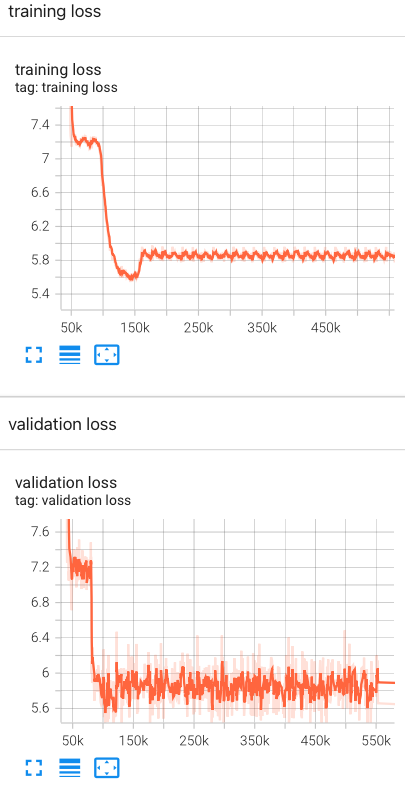
\includegraphics[width=0.45\textwidth]{asset/rnn_tanh.png}}
  \subfigure[LSTM训练曲线]{
  \label{dim1end}
  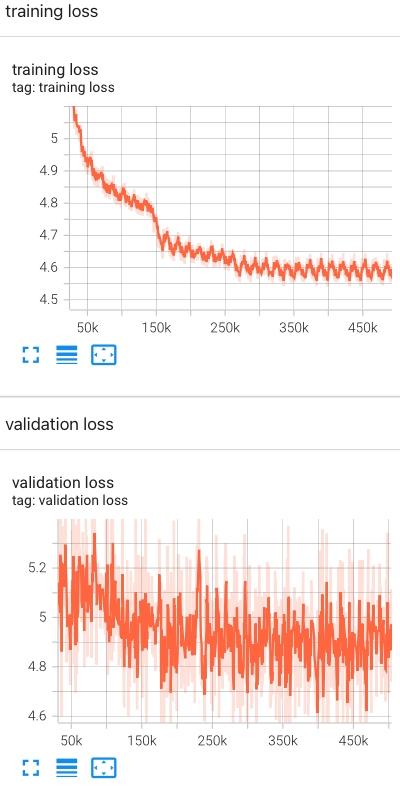
\includegraphics[width=0.45\textwidth]{asset/lstm.png}}
  \caption{Tensorboard结果展示}
  \label{dim1}
\end{figure}

\begin{figure}[htbp]
  \centering
  \subfigure[GRU训练曲线]{
  \label{dim2start}
  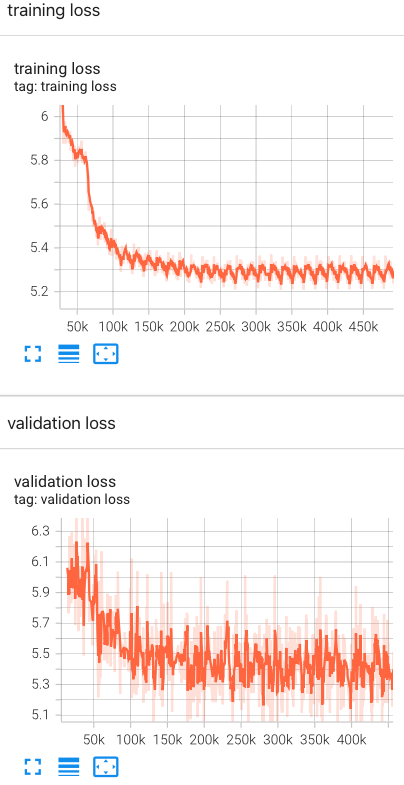
\includegraphics[width=0.45\textwidth]{asset/gru.png}}
  \subfigure[Transformer训练曲线]{
  \label{dim2end}
  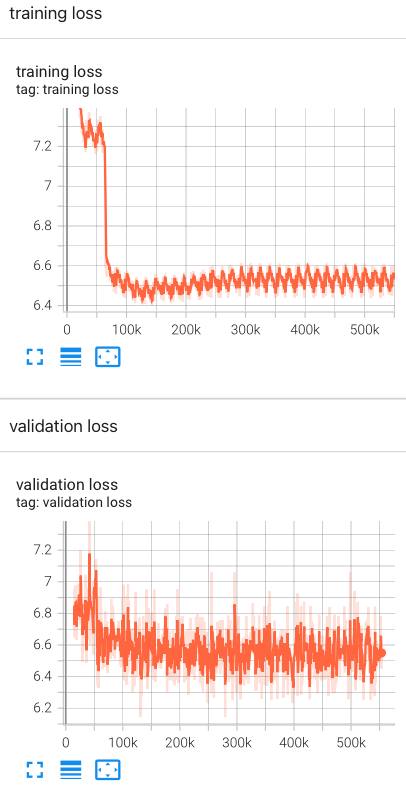
\includegraphics[width=0.45\textwidth]{asset/transformer.png}}
  \caption{Tensorboard结果展示}
  \label{dim2}
\end{figure}

\newpage
\section{总结与思考}

\end{document}

% below is table template used in Deep Learning courses
% \newpage
% \section{总结与思考}

% \begin{table}[H]
%     \centering
%     \begin{tabular}{|c|c|c|c|c|c|c|c|c|c|c|c|c|}
%       \hline
%         \diagbox{评估指标}{参数配置}
%         &\makecell{LR 1e-4\\WD 1e-4}
%         &\makecell{LR 3e-5\\WD 1e-4}
%         &\makecell{LR 5e-5\\WD 1e-4}
%         &\makecell{LR 7e-5\\WD 1e-4}
%         &\makecell{LR 1e-4\\WD 1e-4}
%         &\makecell{LR 1e-4\\WD 2e-4}\\
%         \hline
%         Pretrain&\Checkmark&\Checkmark&\Checkmark&\Checkmark&\XSolidBrush&\XSolidBrush\\
%         \hline
%         Best P.&.9188&.9172&\textbf{.9262}&.9228&.8250&.8393\\
%         \hline
%         Best R.&.9188&.9172&\textbf{.9262}&.9228&.8250&.8393\\
%         \hline
%         Best F1.&.9188&.9172&\textbf{.9262}&.9228&.8250&.8393\\
%         \hline
%         Final P.&.8046&\textbf{.9128}&.8873&.8711&.8003&.7816\\
%         \hline
%         Final R.&.8046&\textbf{.9128}&.8873&.8711&.8003&.7816\\
%         \hline
%         Final F1.&.8046&\textbf{.9128}&.8873&.8711&.8003&.7816\\
%         \hline
%         \diagbox{评估指标}{参数配置}
%         &\makecell{LR 1e-4\\WD 3e-4}
%         &\makecell{LR 1e-4\\WD 7e-5}
%         &\makecell{LR 1e-4\\WD 8e-5}
%         &\makecell{LR 3e-5\\WD 1e-4}
%         &\makecell{LR 5e-5\\WD 1e-4}
%         &\makecell{LR 7e-5\\WD 1e-4}\\
%         \hline
%         Pretrain&\XSolidBrush&\XSolidBrush&\XSolidBrush&\XSolidBrush&\XSolidBrush&\XSolidBrush\\
%         \hline
%         Best P.&.8192&.8170&.8377&.8157&.8335&\textbf{.8426}\\
%         \hline
%         Best R.&.8192&.8170&.8377&.8157&.8335&\textbf{.8426}\\
%         \hline
%         Best F1.&.8192&.8170&.8377&.8157&.8335&\textbf{.8426}\\
%         \hline
%         Final P.&.7965&.8170&\textbf{.8268}&.8073&.7493&.8082\\
%         \hline
%         Final R.&.7965&.8170&\textbf{.8268}&.8073&.7493&.8082\\
%         \hline
%         Final F1.&.7965&.8170&\textbf{.8268}&.8073&.7493&.8082\\
%         \hline
%     \end{tabular}
%     \caption{不同参数配置下的运行结果}
%     \label{fig1}
% \end{table}